\chapter{Language Models e Generative Models}\label{chap:language_models_e_generative_models} % (fold)
\section{Chomsky Grammar Hierarchy}\label{sec:lm_chomsky_grammar_hierarchy} % (fold)
\begin{definition}{Unrestricted Type-0}{lm-unrestricted}
    \textbf{Unrestricted} \textit{Type-0} \hyperref[def:cfg]{Grammars} $G = \pt{V,T,P,S}$, has productions $\al\to\bt \in P$ with $\al\in \pt{V\cup T}^+$ and $\bt\in \pt{V\cup T}^*$.
\end{definition}
\begin{definition}{Context-Sensitive/Monotone Type-1}{lm-monotone}
    \textbf{Context-Sensitive/Monotone} \textit{Type-1} \hyperref[def:cfg]{Grammars} (*) restricts productions to:
    \begin{ceq}
        \al\to\bt\qquad\text{with } |\bt|\ge |\al|
    \end{ceq}
    \begin{example}{}{}
        \begin{ceq}
            \alpha_1A\alpha_2\to\alpha_1\beta\alpha_2
        \end{ceq}
        with $A\in V$, $\beta\in \pt{V\in T}^+$ and $\alpha_1,\alpha_2 \in \pt{V\cup T}^*$.
        \begin{note}
            $\alpha_1,\alpha_2$ are \textbf{not related} to the context
        \end{note}
    \end{example}
\end{definition}
\begin{example}{Monotone Type-1 Grammar}{}
    \begin{ceq}
        \begin{aligned}
            &S\to aSBc|aBc \\
            &cB\to Bc \\
            &aB\to ab \\
            &bB\to bb \\
            & L(G) = \pg{a^nb^nc^n | n\ge 1}
        \end{aligned}
    \end{ceq}
    \begin{itemize}
        \item $S\to aSBc|aBc$ generates $a^n \pt{Bc}^n$ for any $n\ge 1$;
        \item $cB\to Bc$ allows all $B$s to be moved before $c^n$;
        \item $aB\to ab$ turns leftmost $B$ into $b$;
        \item $bB\to bb$ turns other $B$s into $b$ only if adjacent;
    \end{itemize}
\end{example}
\begin{definition}{Context-Free Type-2}{lm-context-free}
    \textbf{Context-Free} \textit{Type-2} \hyperref[def:cfg]{Grammars} (*), has productions $A\to\beta$ with $A\in V$, $\beta\in \pt{V\cup T}^+$
\end{definition}
\begin{definition}{Regular Type-3}{lm-regular}
    \textbf{Regular} \textit{Type-3} \hyperref[def:cfg]{Grammars} (*), has productions $A\to a$ or $A\to aB$ with $A,B\in V$ and $a\in T$.
\end{definition}
\begin{example}{Regular Type-3 Grammar}{}
    \begin{ceq}
        \begin{aligned}
            &S\to aS|a \\
            &L(G) = \pg{a^n | n\ge 1} = \pg{a}^+
        \end{aligned}
    \end{ceq}
\end{example}
\begin{warning}[(*)]
    Also admit a possible $S\to\epsilon$ \textbf{production} for the start symbol $S$ (to represent languages containing $\eps$, provided there is no $\sigma\to\beta \in P$ with $S$ appearing in $\beta$
\end{warning}
\begin{note}
    A grammar $G'$ such that $L(G') = L(G) \cup \pg{\epsilon}$ is obtained from $G = (V,T,P,S)$ by adding a new start symbol $S'$ and productions: $S'\to\epsilon$ and all $S'\to\alpha$ such that $S\to\alpha\in P$
\end{note}
\begin{example}{}{}
    For the Monotone Grammar:
    \begin{ceq}
        \begin{aligned}
            &S'\to aSBc|aBc|\epsilon \\
            &S\to aSBc|aBc \\
            &cB\to Bc \\
            &aB\to ab \\
            &bB\to bb \\
            & L(G) = \pg{a^nb^nc^n | \mathbf{n\ge 0}}
        \end{aligned}
    \end{ceq}
    For the Regular Grammar:
    \begin{ceq}
        \begin{aligned}
            &S'\to aS|a|\epsilon \\
            &S\to aS|a \\
            &L(G) = \pg{a^n | \mathbf{n\ge 0}} = \mathbf{\pg{a}^*}
        \end{aligned}
    \end{ceq}
\end{example}
%
\subsection{Corresponding Language Hierarchy}\label{sub:lm_corresponding_language_hierarchy} % (fold)
\begin{definition}{Semi-Decidable Type-0}{semi-decidable}
    \textbf{Semi-decidable} languages are recognized by a procedure (\textbf{Turing Machine}) that \textbf{halts and accepts} if the input string \textbf{belongs to the language}, otherwise it rejects or does not halt.
\end{definition}
\begin{definition}{Context-Sensitive Type-1}{context-sensitive}
    \textbf{Context-Sensitive} languages are recognized by a \textbf{non-deterministic algorithm} (Turing Machine that always halts) having \textbf{linear space} computational complexity.
\end{definition}
\begin{definition}{Context-Free Type-2}{lm-context-free}
    \textbf{Context-Free} \textit{Type-2} languages are recognized by a non-deterministic \hyperref[def:pda]{Push-Down Automaton}.
\end{definition}
\begin{definition}{Regular Type-3}{lm-regular}
    \textbf{Regular} \textit{Type-3} languages are recognized by a (non-)\hyperref[sub:lr_dfa]{Deterministic Finite State Automaton}.
\end{definition}
\begin{cimage}
    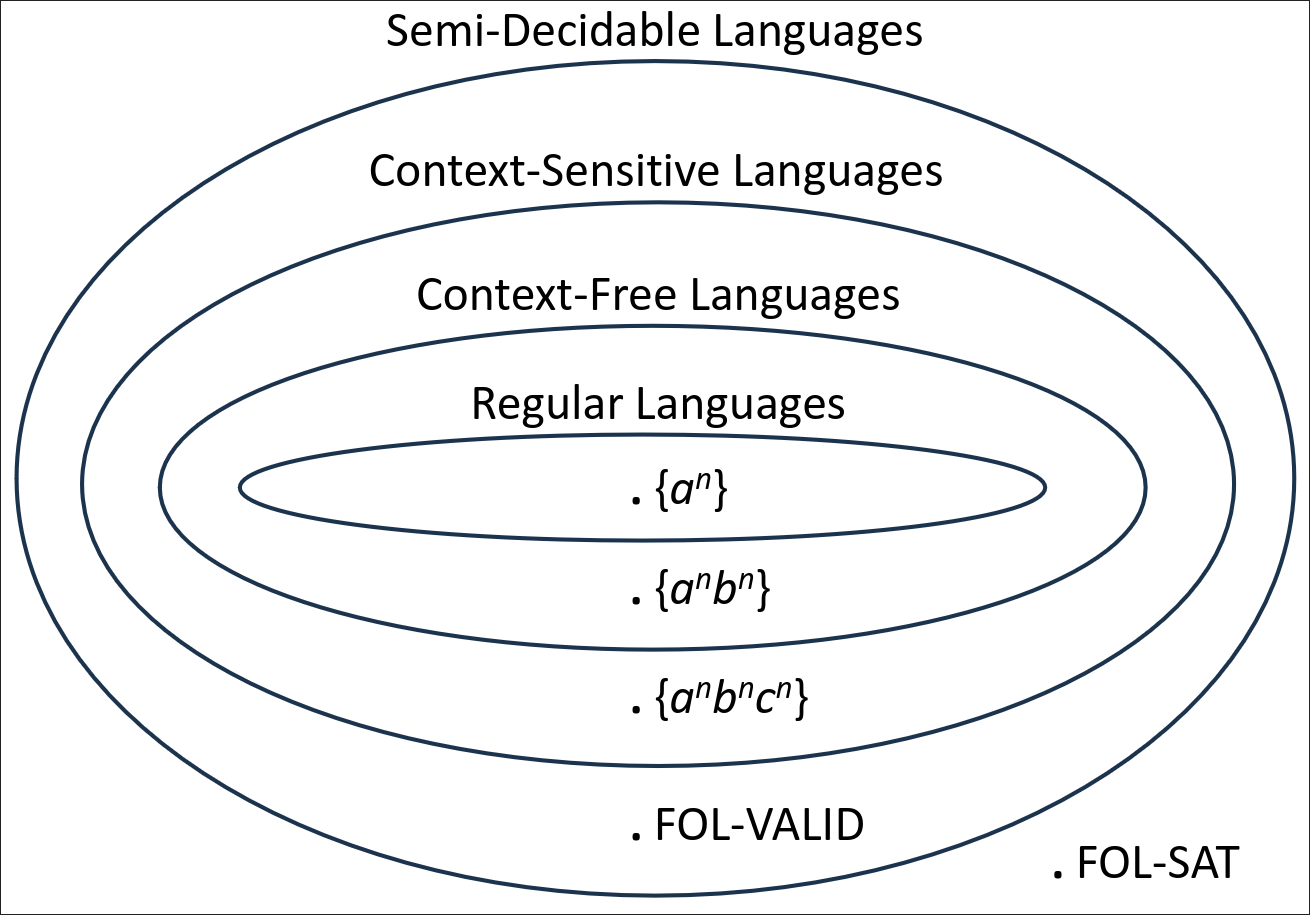
\includegraphics[width=.6\textwidth]{assets/20261105_121407.png}
    \caption{Class-Specific languages}\label{fig:20261105_121407}
\end{cimage}
% subsection Corresponding Language Hierarchy (end)
% section Chomsky Grammar Hierarchy (end)
%
\section{Phrase Structure Grammars}\label{sec:lm_phrase_structure_grammars} % (fold)
Natural languages syntactic categories, such as \textbf{\ac{np}} or \textbf{\ac{vp}}, are \textbf{grammar variables}.
They donate part of sentences which are called \textbf{constituents}.
\begin{note}
    A grammar therefore expresses \textbf{phrase structure}: the relation between \textbf{nodes} (constituency relation) of a \textbf{syntax tree}
\end{note}
\begin{definition}{Tokenization}{tokenization}
    \textbf{Tokenization} is the process of dividing a text into a sequence of words.
    \begin{example}{}{}
        \begin{ceq}
            \text{From the start, it took a person with great qualities to succeed} \\
            \text{From|the|start|,|it|took|a|person|with|great|qualities|to|succeed} \\
        \end{ceq}
    \end{example}
\end{definition}
\begin{definition}{Token}{token}
    A \textbf{token} is a segment of a stream of characters, assuming they belong to a \textbf{finite set}: words that belong to the vocabulary of a language, punctuation, etc.
\end{definition}
Tokens are considered the \textbf{alphabet of symbols} $\Sigma$ used for representing sentences as sequences over $\Sigma$, i.e. strings in $\Sigma^*$.
\begin{example}{}{}
    The sentence:
    \begin{ceq}
        \text{From the start, it took a person with great qualities to succeed} \\
        \text{From|the|start|,|it|took|a|person|with|great|qualities|to|succeed} \\
    \end{ceq}
    is represented by using a \textbf{sequence of tokens} in:
    \begin{ceq}
        \Sigma = \pg{\ps{a},\ps{from},\ps{great},\ps{it},\ps{person},\ps{the},\ps{to},\ps{took},\ps{with},\ps{,},\dots}
    \end{ceq}
    \begin{note}
        Some \textbf{normalization} may happen: e.g. ``From'' and ``from'' are represented by the \textbf{same token} $\ps{from}$.
    \end{note}
\end{example}
\begin{definition}{Ambiguity}{lm-ambiguity}
    Natural languages are \textbf{ambiguous}: it is normal for a sentence to have several different syntax trees.
\end{definition}
\begin{example}{}{}
    Consider the \hyperref[def:cfg]{CFG}:
    \begin{ceq}
        \begin{aligned}
            &S\to NP\ VP \\
            &NP \to Noun\ |\ Pronoun \\
            &VP \to Verb\ NP\ |\ Modal\ Verb \\
            \\
            &Noun \to \ps{fish}\ |\ \dots \\
            &Pronoun \to \ps{I}\ |\ \ps{they}\ |\ \dots \\
            &Verb \to \ps{can}\ |\ \ps{fish}\ |\ \dots \\
            &Modal \to \ps{can}\ |\ \dots \\
        \end{aligned}
    \end{ceq}
    The sentence ``I can fish'' has two syntax:
    \begin{cimage}
        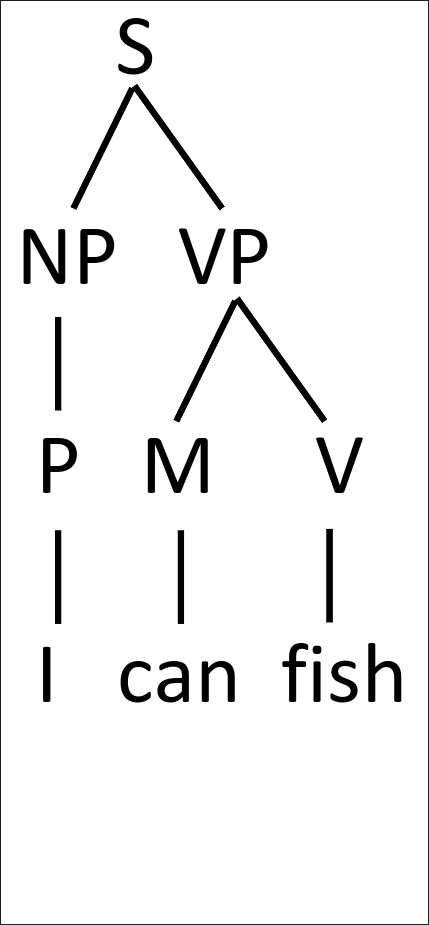
\includegraphics[width=.2\textwidth]{assets/20261105_134957.png}
        $\qquad\qquad$
        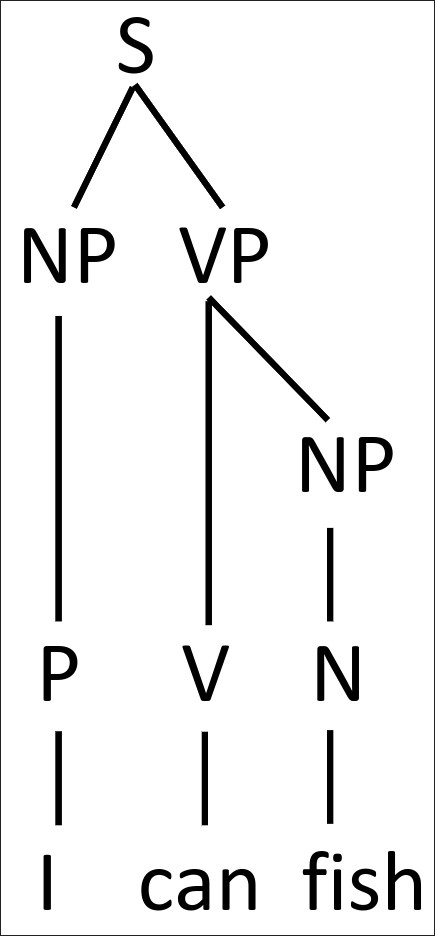
\includegraphics[width=.2\textwidth]{assets/20261105_135042.png}
    \end{cimage}
\end{example}
\begin{remark}{}{}
    \hyperref[def:lm-ambiguity]{Ambiguity} is handled using a \red{probabilistic} approach, by \textit{assigning probabilities} to grammar productions (e.g. to select the \red{most probable} syntax tree).
\end{remark}
% section Phrase Structure Grammars (end)
% chapter Language Models e Generative Models (end)
